%%%%%%%%%%%%%%%%%%%%%%%%%%%%%%%%%%%%%%%%%%%%%%%%%%%%%%%%%%%%%%%%%%%%%%%%%%%%%%%%%%%%%%%%%%%%%%
% --一些基本设置,各种包的扩展--
%%%%%%%%%%%%%%%%%%%%%%%%%%%%%%%%%%%%%%%%%%%%%%%%%%%%%%%%%%%%%%%%%%%%%%%%%%%%%%%%%%%%%%%%%%%%%%
% A4纸张大小
\documentclass[UTF8,a4paper,10pt]{ctexart}
% 页边距
\usepackage[left=2.50cm, right=2.50cm, top=2.50cm, bottom=2.50cm]{geometry}
% 设置章标题居左
\CTEXsetup[format={\Large\bfseries}]{section} 
%%%%%%%%%%%%%%%%%%%%%%%%%%%%%%%%%%%%%%%%%%%%%%%%%%%%%%%%%%%%%%%%%%%%%%%%%%%%%%%%%%%%%%%%%%%%%%
% -- 专门设置页眉页脚 --
%%%%%%%%%%%%%%%%%%%%%%%%%%%%%%%%%%%%%%%%%%%%%%%%%%%%%%%%%%%%%%%%%%%%%%%%%%%%%%%%%%%%%%%%%%%%%%
\usepackage{fancyhdr}
\pagestyle{fancy}
% bfseries
% 页眉
\lhead{}
\chead{社交媒体用户的音乐推荐}
\rhead{}
% 页脚
\lfoot{}
\cfoot{第 \thepage 页}
\rfoot{}
% 修改格式
\renewcommand{\headrulewidth}{0.4pt}
\renewcommand{\footrulewidth}{0.4pt}
%%%%%%%%%%%%%%%%%%%%%%%%%%%%%%%%%%%%%%%%%%%%%%%%%%%%%%%%%%%%%%%%%%%%%%%%%%%%%%%%%%%%%%%%%%%%%%
% -- 设置字体 --compile using Xelatex
%%%%%%%%%%%%%%%%%%%%%%%%%%%%%%%%%%%%%%%%%%%%%%%%%%%%%%%%%%%%%%%%%%%%%%%%%%%%%%%%%%%%%%%%%%%%%%
% -- 中文字体 --
%\setmainfont{Microsoft YaHei}  % 微软雅黑
%\setmainfont{YouYuan}  % 幼圆    
%\setmainfont{NSimSun}  % 新宋体
%\setmainfont{KaiTi}    % 楷体
%\setmainfont{SimSun}   % 宋体
%\setmainfont{SimHei}   % 黑体
% -- 英文字体 --
\usepackage{times}
%\usepackage{mathpazo}
%\usepackage{fourier}
%\usepackage{charter}
%\usepackage{helvet} 
%%%%%%%%%%%%%%%%%%%%%%%%%%%%%%%%%%%%%%%%%%%%%%%%%%%%%%%%%%%%%%%%%%%%%%%%%%%%%%%%%%%%%%%%%%%%%%
% --设置水印--
%%%%%%%%%%%%%%%%%%%%%%%%%%%%%%%%%%%%%%%%%%%%%%%%%%%%%%%%%%%%%%%%%%%%%%%%%%%%%%%%%%%%%%%%%%%%%%
% 所有页加水印
%\usepackage{draftwatermark}
% 只有第一页加水印         
%\usepackage[firstpage]{draftwatermark}
% 设置水印内容 
%\SetWatermarkText{Water-Mark}
% 设置水印logo           
%\SetWatermarkText{\includegraphics{fig/ZJDX-WaterMark.eps}}
% 设置水印透明度 0-1         
%\SetWatermarkLightness{0.9}
% 设置水印大小 0-1             
%\SetWatermarkScale{1}
%%%%%%%%%%%%%%%%%%%%%%%%%%%%%%%%%%%%%%%%%%%%%%%%%%%%%%%%%%%%%%%%%%%%%%%%%%%%%%%%%%%%%%%%%%%%%%
% --用于标注代码的样式--
%%%%%%%%%%%%%%%%%%%%%%%%%%%%%%%%%%%%%%%%%%%%%%%%%%%%%%%%%%%%%%%%%%%%%%%%%%%%%%%%%%%%%%%%%%%%%%                     
\usepackage{listings} 
\lstset{						 % 下面是一些设置
  language=python,               % 代码语言
  basicstyle=\footnotesize,      % 代码的尺寸大小
  numbers=left,                  % 将行号写到左边
  numberstyle=\tiny\color{gray}, % 行号的风格
  stepnumber=2,                  % 行与行的间隔标号,如果为1,则每一行都会被标记行号
  numbersep=5pt,                 % 行号与代码之间的间距
  backgroundcolor=\color{white}, % 如果选择背景色,你必须加 \usepackage{color},color可以是其他色
  showspaces=false,              % show spaces adding particular underscores
  showstringspaces=false,        % underline spaces within strings
  showtabs=false,                % show tabs within strings adding particular underscores
  frame=single,                  % adds a frame around the code
  rulecolor=\color{black},       % if not set, the frame-color may be changed on line-breaks 									within not-black text (e.g. commens (green here))
  tabsize=2,                     % sets default tabsize to 2 spaces
  captionpos=b,                  % sets the caption-position to bottom
  breaklines=true,               % sets automatic line breaking
  breakatwhitespace=false,       % sets if automatic breaks should only happen at whitespace
  title=\lstname,                % show the filename of files included with \lstinputlisting;
                                 % also try caption instead of title
  keywordstyle=\color{blue},     % keyword style
  commentstyle=\color{dkgreen},  % comment style
  stringstyle=\color{mauve},     % string literal style
  escapeinside={\%*}{*)},        % if you want to add LaTeX within your code
  morekeywords={*,...}           % if you want to add more keywords to the set
}
%%%%%%%%%%%%%%%%%%%%%%%%%%%%%%%%%%%%%%%%%%%%%%%%%%%%%%%%%%%%%%%%%%%%%%%%%%%%%%%%%%%%%%%%%%%%%%
%%%%%%%%%%%%%%%%%%%%%%%%%%%%%%%%%%%%%%%%%%%%%%%%%%%%%%%%%%%%%%%%%%%%%%%%%%%%%%%%%%%%%%%%%%%%%%
% --其他可用的建设性模板(仅供复制修改)--
%%%%%%%%%%%%%%%%%%%%%%%%%%%%%%%%%%%%%%%%%%%%%%%%%%%%%%%%%%%%%%%%%%%%%%%%%%%%%%%%%%%%%%%%%%%%%%                    
%%%%%%%%%%%%%%%%%%%%%%%%%%%%%%%%%%%%%%%%%%%%%%%%%%%%%%%%%%%%%%%%%%%%%%%%%%%%%%%%%%%%%%%%%%%%%%
% --用于创建表格--
%\begin{table}[htbp]
%		\caption{Title of table} \label{tab:table}
%		\centering
%		\addtolength{\tabcolsep}{-0mm} % 控制列间距
%		\begin{tabular}{ccccc}
%			\toprule[0.75pt]	% package booktabs
%			\multicolumn{4}{c}{table head} \\
%			\midrule[0.5pt]	% package booktabs
%			\multirow{4}{*}{text} & 1 & 2 & 3 & 4 \\  % package multirow
%			& 5 & 6 & 7 & 8 \\
%			\cmidrule[0.5pt]{2-4}	% package booktabs
%			& 9 & 10 & 11 & 12 \\
%			& 13 & 14 & 15 & 16 \\
%			\bottomrule[0.75pt]	% package booktabs
%		\end{tabular}
%\end{table}
%%%%%%%%%%%%%%%%%%%%%%%%%%%%%%%%%%%%%%%%%%%%%%%%%%%%%%%%%%%%%%%%%%%%%%%%%%%%%%%%%%%%%%%%%%%%%%
% --写个算法伪代码流程图--
%\begin{algorithm}
%		\caption{Title of the Algorithm}
%		\label{algo:ref}
%		\begin{algorithmic}[1]
%			\REQUIRE some words.  % this command shows "Input"
%			\ENSURE ~\\           % this command shows "Initialized"
%			some text goes here ... \\
%			\WHILE {\emph{not converged}}
%			\STATE ... \\  % line number at left side
%			\ENDWHILE
%			\RETURN this is the lat part.  % this command shows "Output"
%		\end{algorithmic}
%\end{algorithm}
%%%%%%%%%%%%%%%%%%%%%%%%%%%%%%%%%%%%%%%%%%%%%%%%%%%%%%%%%%%%%%%%%%%%%%%%%%%%%%%%%%%%%%%%%%%%%%
%%%%%%%%%%%%%%%%%%%%%%%%%%%%%%%%%%%%%%%%%%%%%%%%%%%%%%%%%%%%%%%%%%%%%%%%%%%%%%%%%%%%%%%%%%%%%%

\usepackage{color}
\usepackage{cite}

\definecolor{dkgreen}{rgb}{0,0.6,0}
\definecolor{gray}{rgb}{0.5,0.5,0.5}
\definecolor{mauve}{rgb}{0.58,0,0.82}


 
\usepackage{amsmath, amsfonts, amssymb} % math equations, symbols
\usepackage[english]{babel}
\usepackage{color}      % color content
\usepackage{graphicx}   % import figures
\usepackage{url}        % hyperlinks
\usepackage{bm}         % bold type for equations

\usepackage{multirow}
\usepackage{booktabs}
\usepackage{epstopdf}
\usepackage{epsfig}
\usepackage{algorithm}
\usepackage{algorithmic}
\usepackage{subfigure}
\usepackage{pdfpages}

% use Input in the format of Algorithm
\renewcommand{\algorithmicrequire}{ \textbf{Input:}}
% use Initialize in the format of Algorithm       
\renewcommand{\algorithmicensure}{ \textbf{Initialize:}} 
% use Output in the format of Algorithm  
\renewcommand{\algorithmicreturn}{ \textbf{Output:}}       
 
 
 
 
  
% 超链接
%\usepackage{hyperref} %bookmarks
%\hypersetup{colorlinks, bookmarks, unicode} %unicode
% 
% 
% 


%%%%%%%%%%%%%%%%%%%%%%%%%%%%%%%%%%%%%%%%%%%%%%%%%%%%%%%%%%%%%%%%%%%%%%%%%%%%%%%%%%%%%%%%%%%%%%
% --正文如下--
%%%%%%%%%%%%%%%%%%%%%%%%%%%%%%%%%%%%%%%%%%%%%%%%%%%%%%%%%%%%%%%%%%%%%%%%%%%%%%%%%%%%%%%%%%%%%%
%% 一些前期工作
% 文章题目
% \title{\textbf{社交媒体用户的音乐推荐文献综述}}
% \title{\textbf{社交媒体用户的音乐推荐实验方案设计}}
%\title{\textbf{社交媒体用户的音乐推荐程序说明与系统性能报告}}
\title{\textbf{社交媒体用户的音乐推荐实验方案改进说明}}
% \title{\textbf{社交媒体用户的音乐推荐}}
% 作者
\author{ 计63 肖朝军 2016011302 \\ 计63 曹晨阳 2015010603 \\ 计63 张泽阳 2016010425} %\thanks{学号:2016310200112} }
% 日期(还没想到怎么删)
%\date{\today}
%%%%%%%%%%%%%%%%%%%%%%%%%%%%%%%%%%%%%%%%%%%%%%%%%%%%%%%%%%%%%%%%%%%%%%%%%%%%%%%%%%%%%%%%%%%%%%
\begin{document}
    \maketitle %输出标题
        
 
%\newpage%另起一页
% \begin{abstract}
% 文献综述就不要摘要了

%\centering
% \textbf{关键字:}关键词1 关键词2
% \end{abstract}
\thispagestyle{empty}


\tableofcontents
\clearpage
%标题栏
%\section{文献综述}
%\section{背景}
% 介绍推荐发展的历史,以及为什么要有社交媒体的推荐


%\subsection{音乐推荐系统分析}
虽然音乐推荐系统是推荐系统的一个小部分,但是由于歌曲和收听用户自身的一些特性,音乐推荐系统和其他推荐系统还是有一些不同点的\cite{MusicComSurvey},比如与电影,书籍,新闻等推荐系统。在此部分中,我们将对于这些音乐推荐系统特性,面临的挑战与发展方向进行一定的分析。

\subsubsection{音乐推荐系统的特性}
首先,分析一下音乐及其推荐系统不同于其他推荐任务的特性\cite{MusicComFeature};
\paragraph{时长}
我们对于一个物品或一项内容的感觉与我们接触它的时长时有一定关系的,从时长上来看,通常的电影持续约90分钟或者更长,而对于书籍我们通常要花费若干小时,若干天甚至一周以上的时间来进行阅读。而对于音乐,大部分的流行音乐的时长都在3分钟到5分钟的时间内,而可能存在一些古典音乐,其时长会有更长,但是相比于电影或者是书籍,仍然有一些差距\cite{MusicComSurvey}。因此,较小的持续时长也就导致了音乐表现出更多的“可丢弃”的性质。

\paragraph{数量}
推荐系统也受到其可供推荐的内容多少的限制。对于电影推荐系统的话,根据Netflix在2016年的数据,其电影和电视剧的总数约为5500;而对于书籍推荐系统,亚马逊在2017年的书籍数量为4000万左右;对于音乐推荐,根据Spotify在2017年的数据,报告了约3000万首歌曲。\cite{MusicComSurvey}可见相较于电影推荐系统,歌曲的推荐的集合要大的多,这就要求音乐推荐系统必须拥有更加高效的方法来对于如此庞大的数据进行分析处理。

\paragraph{连续}
用户在听歌时,一次可能会听很多首歌,或者说用户的听歌行为很少是面向于单曲的,而更像是面向于歌单、专辑或者歌手的。所以这种连续的收听与电影或者书籍的推荐系统又有了一些不同。

\paragraph{重复}
对于电影来讲,大部分电影我们在一段时间内可能不会去看很多遍,除非我们对于这个电影有极大的偏爱。但是此时就算推荐系统不给我们推荐我们也会去看,所以在这里不存在重复推荐的问题。但是对于歌曲推荐系统而言,歌曲推荐是存在重复推荐的,那么两次推荐之间的时间间隔应该怎样选取,怎样的音乐适合于进行重复推荐等问题也就相应产生了。

\paragraph{目的}
音乐对于用户来讲,其实是有多种功能的,例如我们可能会在打牌时选择播放“斗地主”的背景音乐来活跃气氛,或者为了哄家里的小孩子放一些儿童向的歌曲。这些播放行为通常带有更多的是我们的目的性,而非我们个人对于这类歌曲有更大的偏爱。所以能否正确辨别这些情况,能够很大地改善用户在使用推荐系统时的体验。此外,有研究人员对于听音乐的目的在社会学的角度上也提供了一些研究\cite{MusicUses}。

\paragraph{心境}
音乐与人内心的情感是密不可分的,相同的人在不同的心情下可能会选择不同的歌曲来听\cite{EmotionInflunce}。所以音乐推荐系统会更加依赖于对于用户情感的分析。同时,音乐对于人的心情也有相互的作用,有些时候我们可能需要音乐来为我们“助兴”,而有些时候我们可能需要音乐来帮助我们放松心情,减轻压力等。这种基于用户心境的推荐是音乐推荐系统中比较关键且富有挑战性的内容。

\paragraph{场景}
与心情类似,场景也是决定我们决定听歌内容的一大影响因素\cite{SituationalInflunce}。如果能够根据用户的地理位置,将这部分信息纳入到音乐推荐的评估当中,也能够提高用户的使用体验\cite{LocationalInflunce}。

\subsection{音乐推荐系统的挑战}
在音乐推荐的过程当中,存在一些独特的,且影响较大的问题\cite{Challange}:

\paragraph{冷启动}
冷启动指的是在没有足够多的用户数据的时候如何对于新用户正常地进行音乐推荐,或者对于新上架的歌曲,没有更多的评价信息,如何将其正确地推荐给用户。冷启动的问题在很多的推荐系统当中是一个普遍存在的问题\cite{ColdStart},但是对于音乐推荐系统来讲,其短时间,多数量的性质导致了这种冷启动的问题很严重。这种冷启动还可能带来的一个问题就是数据的稀疏性,对于一个用户来讲,其未评分的歌曲数远大于其进行过评分的歌曲数。当这种稀疏性过大时,可能会导致推荐系统不准确\cite{Challange}。

\paragraph{自动播放列表}
在上面的特性中可以看出,用户在听歌时经常以一个歌单为基本的形式。所以如何自动生成、维护和推荐歌单就是推荐系统需要考虑的又一大问题。同时,在歌单内部歌曲之间是否具有一定的共同特征,以及歌曲之间的相互衔接对于歌单的质量也会造成一些影响\cite{Context}。在歌单的基础上,歌单与歌单之间的关联与推荐,歌单的冷启动问题,也有一些值得去处理的问题。

\paragraph{评估标准}
在机器学习以及其他相关领域中,已经发展出一系列用于评估性能的参数,在音乐推荐系统中也有较大的效用。这部分内容将在后面进行更加详细的介绍。

\subsubsection{发展前景}
\paragraph{基于用户心理的音乐推荐}
在上面的特性中可以看出,用户的心情对于其音乐的选择是起到很大的影响的\cite{EmotionInflunce}。在传统的方法中,我们用到的更加普遍的方法是根据用户的历史行为,以及一些个人的背景资料,来完善推荐系统对于人的个性化需求的处理。所以对于音乐推荐系统,其一大改进方向就是通过一些用户数据,推测用户当前的心理状态,在此基础上结合其他特征进行音乐的推荐。

\paragraph{基于场景的音乐推荐}
一般的推荐系统的重点均为根据用户以及音乐的相关内容,来求出推荐内容。但是在真实的生活场景中,一些在用户和音乐之外的因素同样能够对于音乐的推荐造成比较大的影响,就如时间\cite{TimeInflunce},地点\cite{Location},季节\cite{Season}等。所以基于场景的音乐推荐能够综合考虑用户实在什么样的场合下播放的音乐,从而能够推荐更加符合当前场景的音乐。

\paragraph{基于文化背景的音乐推荐}
个人的兴趣爱好和选择偏向已经在推荐系统中被高效地利用且有着不错的表现,但是更高层次地,用户所在的文化氛围从一定程度上决定了用户一部分的选择偏向\cite{Culture},所以如果能够现根据用户的文化背景进行一个粒度较粗的分类,再在此基础上进行细分,可以提升系统的准确程度。
%\section{基于神经网络的推荐算法}
%\section{推荐系统评价指标}

%\section{推荐系统的评价指标}
%\subsection{文献综述总结}
基于文献的阅读和总结,我们初步了解了推荐系统的实现方法和发展历程,包括早期的传统方法和之后的神经网络方法。在调研过程中,我们发现,神经网络方法确实能够比传统方法有更高的性能,所以我们下一步的思路更倾向于进一步发掘神经网络方法在社交媒体用户的音乐推荐上的应用。但是,这也带来了一些潜在的问题,比如可解释性等,这些问题也是我们在下一步研究中重点关注的部分。经过讨论,我们对于研究方向的初步展望有如下几个方向:
\begin{itemize}
    \item 可解释的推荐系统:为了解决神经网络方法在可解释性上的缺陷,可以对于如何在可解释性上进行进一步的研究,从而提高模型的性能。
    \item 推荐系统的推理能力:由于我们拿到了一系列用户在听歌这一行为之外的数据,如朋友圈的发文等,所以我们希望能够从这些信息中,推理出用户的更多信息,来进行精度更高的推荐。
    \item 跨领域推荐:不同的推荐系统之间,从某种程度上是可以有一定的交互的。因为两者都在一定程度上依赖于用户本身的特征,所以一种可能的方向就是根据其他推荐系统的结果,来进行音乐推荐。
\end{itemize}
更加详细的研究计划将在后面一周的讨论中逐步进行完善和初步构建。
%\section{实验方案设计}
%\subsection{深入调研——冷启动问题}
在之前的文献综述过程中,我们较为详细地讨论了推荐系统的发展过程,以及实现的方法与模型。但是对于推荐问题,仍然有一些潜在的问题,可能会较大地影响推荐系统的结果\cite{currentprob}。其中一大问题就是冷启动问题。冷启动问题在音乐推荐系统中表现地尤为明显,由于音乐的数量很大,用户对于音乐的评分矩阵往往是稀疏的。所以音乐推荐系统中,冷启动的影响是较大的。所以我们首先对于这一问题的解决方法进行了更深入的探究。

\subsubsection{冷启动问题的分类}
在现有的研究中,研究者将冷启动问题进行细分,分成了两部分问题。一类是CCS,表示用户或者音乐完全是新的,没有历史的交互数据,这就导致了部分的模型是完全不工作的。另一类是ICS,表示用户或音乐是有一部分交互信息的,但是这部分的交互信息对于描述用户评分特征上来看是不够充分的,此时给出的推荐结果也是不可靠的,可能会影响到用户的使用体验。

\subsubsection{冷启动问题的相关工作}
对于推荐系统中的冷启动问题,已经有了一部分相关的工作,来解决这一问题。具体的解决方法有如下几种\cite{currentprob}:
\begin{itemize}
    \item Content-Based方法
    \item 混合模型
    \item Cross-Domain模型
    \item Active Learning
\end{itemize}

这四种方法的主要思路大体是相似的,都是利用用户和音乐的其他信息来对于交互项进行补充,从而加强对于用户和音乐特征的建模。

此外,从推荐系统之外的领域,也有一些关于缺失数据的处理过程可供借鉴。比如图片分类问题,一些完全没有见过的图片,我们需要对其进行分类的问题为Zero-Shot的问题,而对于一些出现次数较少的图片,其分类问题为Few-Shot问题。这两种问题中,Zero-Shot问题可以和推荐问题中的CCS问题对应,而Few-Shot问题可以与推荐问题中的ICS问题对应。所以我们可以参考图片分类问题中对于Few-Shot问题和Zero-Shot问题的处理,给出相似的解决方案\cite{currentprob}。

\begin{figure}[htb]        
\center{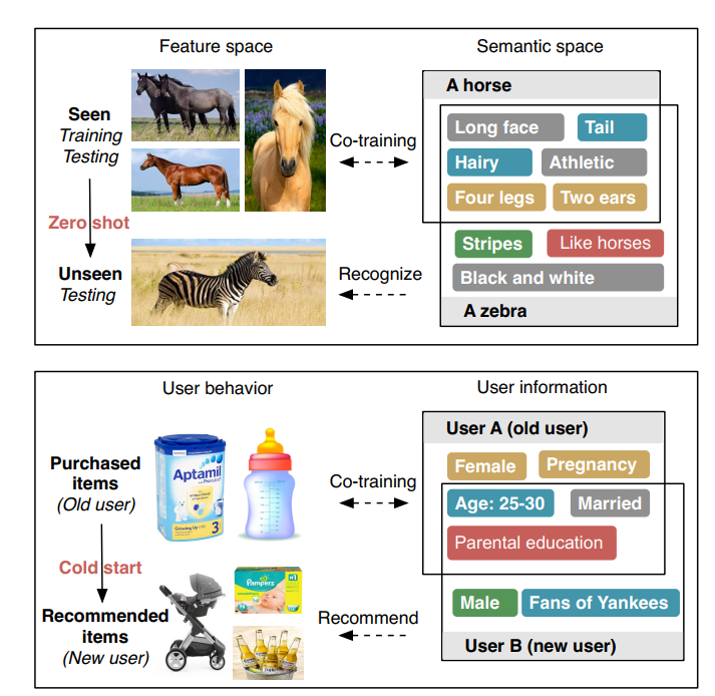
\includegraphics[width=10cm]  {MusicRecomSurvey/pics/zero-shot.png}}    
\caption{\label{1} Zero-Shot方法}      
\end{figure}

\begin{figure}[htb]        
\center{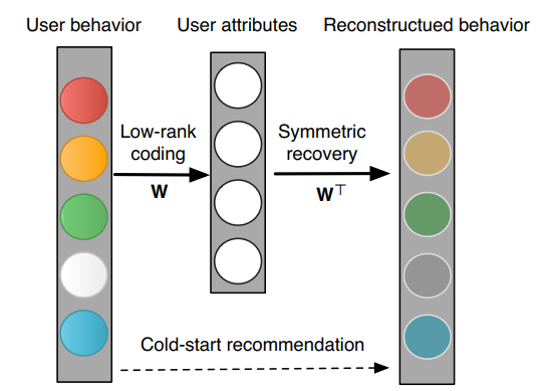
\includegraphics[width=8cm]  {MusicRecomSurvey/pics/autoencoder.png}}    
\caption{\label{2} AutoEncoder方法}      
\end{figure}
一种方法是使用用户信息及物品信息,如图1所示,如果我们能够采集有效的信息,就可以在此基础上进行一定的推断,得出用户对于一些物品的喜爱程度。在此基础上,可以更进一步,使用AutoEncoder的结构,对于特征进行提取,如图2所示。此时对于冷启动的用户,通过AutoEncoder先进行编码,再进行解码,则最后解码得到的值就包含了该用户在这里通过用户特征推测出的值\cite{zeroshot}。

另一种方法将这一问题转化为了Meta-Learning的问题,使用Meta-Learning的方法来解决冷启动的问题\cite{metalearning}。如图3所示。
\begin{figure}[htb]        
\center{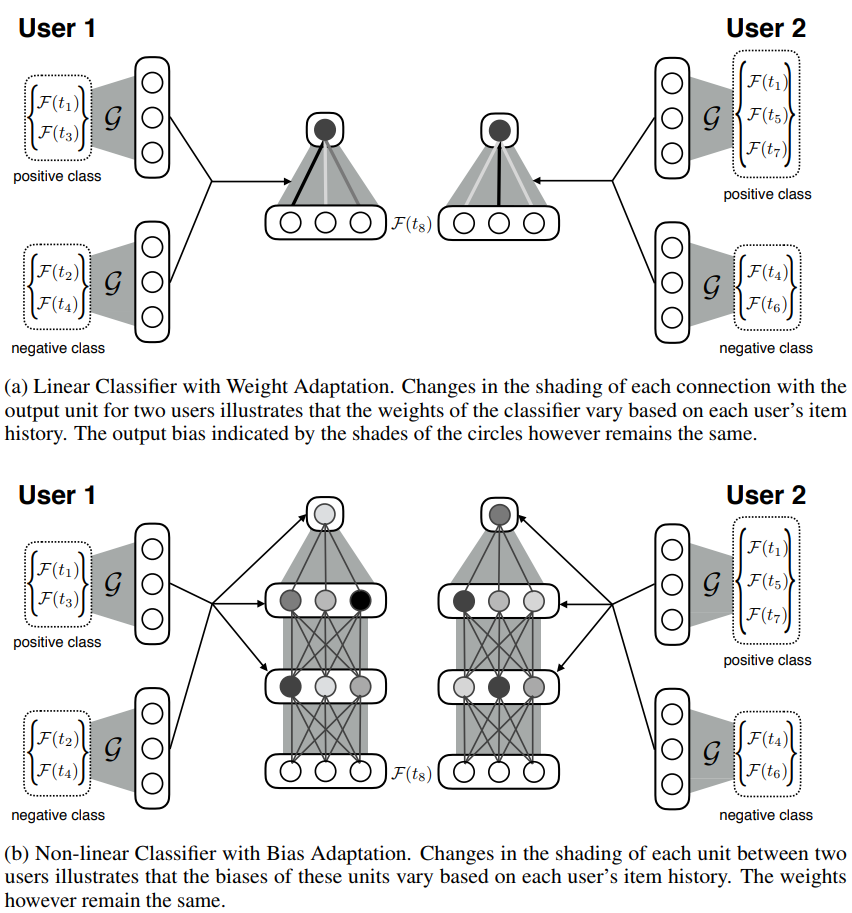
\includegraphics[width=8cm]  {MusicRecomSurvey/pics/meta.PNG}}    
\caption{\label{3} Meta-Learing方法}      
\end{figure}

\subsubsection{我们的研究思路}
在调研过程中,我们发现对于冷启动问题,CCS和ICS两个子问题在解决方法上也存在一定的差异\cite{coldstart},所以我们认为不一定要设计出一个模型,来对两个子问题都找到较好的解法。所以我们在设计自己的模型时更加注重于对于ICS问题。希望能尽可能高效地利用有限的评分信息,对于用户的评分习惯进行更准确的分析。

同时,借鉴了CV领域中的Relation-Learning的思想,我们希望能够使得推荐系统能够通过一种更加准确的方式来学会如何“比较相似性”。在此基础上,我们调研了在推荐系统中运用Metric-Learning的情况,发现虽然这些方法已经初步有了使推荐系统学习距离信息来推测相似度的相关想法,但是其优化的距离或者说用于定义相似度的距离都是低阶线性的距离算法。这种方法虽然可以给出一定的距离描述,但是难以对于神经网络提取的高阶特征进行充分的捕捉和利用。所以我们希望能够通过Relation-Learning中计算图片与图片之间相似度的方法,应用到推荐系统中用于计算人与人,音乐与音乐,用户与音乐之间交互等的相似性。

所以我们的模型的基本思路就确定为一个混合推荐模型,使用Relation-Learning的思路,学习用户评分的相似性,之后通过协同过滤,对于评分的值进行估计。
%\subsection{模型设计}
\subsubsection{模型思路}
我们的模型的核心是度量相似度。
相似度的作用在协同过滤算法中有着诸多的体现,协同过滤算法通过用户与用户之间在评分行为上的相似性,或者歌曲与歌曲在得分上的相似性,来对于未知的评分进行估计。我们的模型也希望能够通过一种更加优良的方法来获取这种相似度信息。
同时,根据之前的分析,我们希望能够提取出用户和歌曲的高阶非线性信息,而传统方法中获取相似度时,用到的还是低阶线性的信息,所以我们就按照这种思路,希望能够通过高阶非线性特征来描述用户在评分行为上的相似性。
接下来,就是如何定义这里的相似性。我们对于这样相似性的定义为:对于用户$u_a$,已经评价过一系列歌曲$m_1, \cdots, m_k$,这样的评分行为与对于未知歌曲$m$的评分行为之间的相似性,所以这种评分行为很大程度上参考了歌曲之间的高阶相似度,同时也将用户特征纳入了考虑范围之内。
在得到高阶非线性相似度之后,我们来对于这样的相似度进行进一步的处理,得到评分预测。这里的思路就和传统的协同过滤有一定的相似程度,但是考虑到一些情况,我们对于这样的过程进行了一些修正,具体的结构和实现在后面进行详细描述。

\subsubsection{模型结构}
我们设计了如图7所示的模型:
\begin{figure}[htb]        
\center{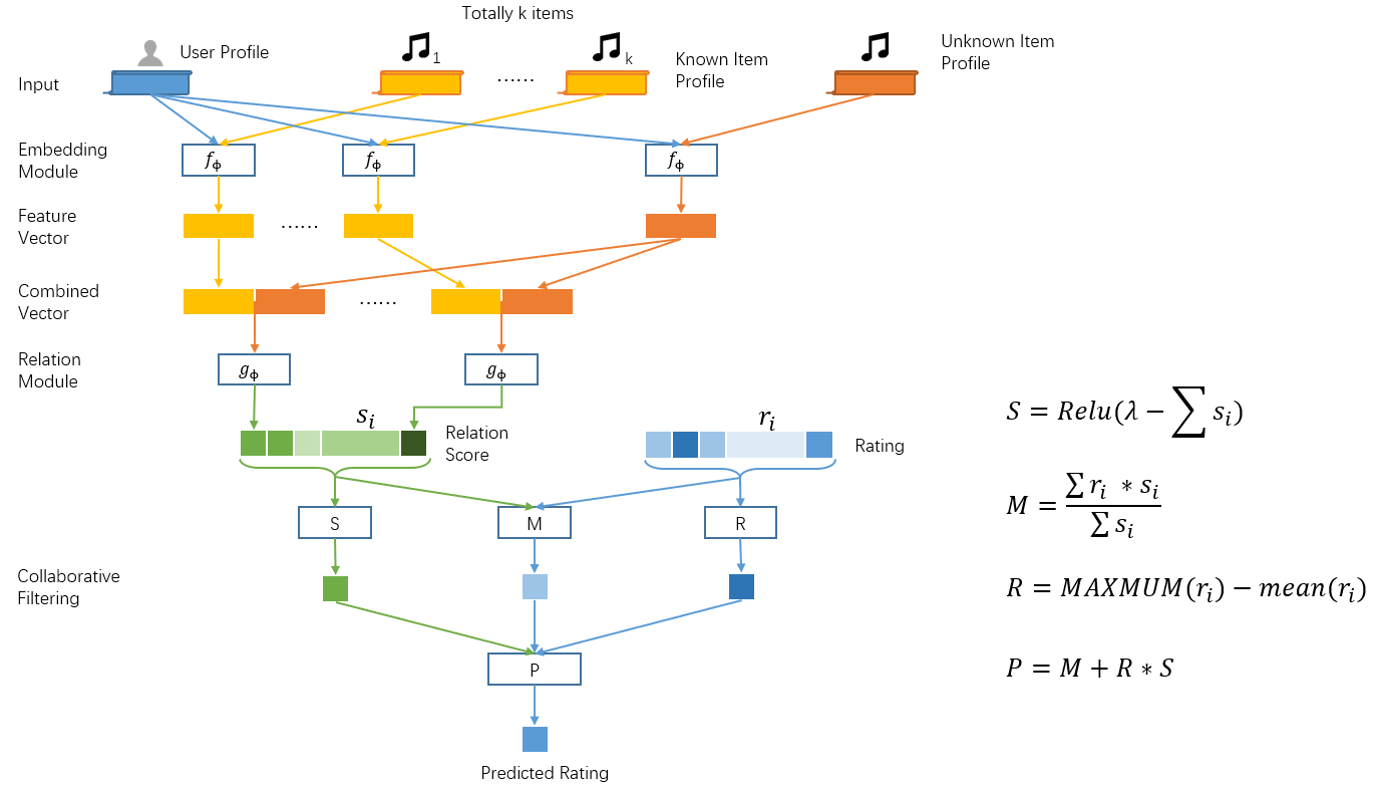
\includegraphics[width=15cm]  {MusicRecomSurvey/pics/model.PNG}}    
\caption{\label{4} 模型结构图}      
\end{figure}

\paragraph{输入}
模型的输入主要包含两部分:一部分是特征信息,包含目标用户的特征信息、已经评分的$k$首歌曲的特征信息以及目标歌曲的特征信息。另一部分是评分信息,包含了目标用户对于$k$首已经评分歌曲的评分值。

\paragraph{Embedding Module}
由于我们获取的特征信息并不是形式化的向量值,所以需要对其进Embedding从而对于特征进行提取。而我们在这里的一个设计是将用户特征和音乐特征结合其来进行Embedding处理。因为我们认为不同的人对于音乐有不同的偏好,所以在提取特征时,如果只对于音乐特征进行特征提取和描述,则无法体现出不同用户对于这些音乐的交互特征。所以我们在进行特征提取时,就将两者的特征进行了整合。如图中$f_{\phi}$模块所示,其输入为目标用户的信息和音乐的信息,输出为对于两者进行组合和编码后,得到的向量化的用户评分行为的特征信息。这里可用的方法有很多种,可以使用AutoEncoder模型来完成特征提取,也可以使用其他的特征提取方法。

\paragraph{Relation Module}
在上一部分中,我们将数据集中关于用户和音乐的信息进行处理,得到了其高阶非线性特征向量作为输出。在下一部分的模型中,我们希望能通过这样的特征,给出用户对不同的音乐之间的评分相似性给出一个评价。我们首先将用户对于已评分歌曲的特征和目标未评分歌曲的特征进行组合,表示比较相关性的两个歌曲特征,之后通过比较相似性的模块$g_{\phi}$来给出两者之间的相似性,并通过归一化函数将其大小限定在0到1之间,最终得到一个$k$维的数值向量Relation Score。

\paragraph{协同过滤}
在上面的输出中,我们得到了用户对未知歌曲的评价,与一些已知歌曲评分的相似性。之后就可以借助协同过滤方法对于目标用户对目标歌曲的评分进行估计。同时,为了更好地对于用户的评分进行预测,我们对于传统的估计方式进行了改进,使其能够对于ICS的情况具有更好的普适性和准确度。
首先额外输入用户对于这些已评价歌曲的评分$Rating$,结合之前得到的$Relation Score$,可以求出参数$M$,即传统的协同过滤当中根据相似度进行加权平均之后的估计值。我们通过另外两项参数$S$和$R$来对这个估计值进行修正。
我们通过参数$S$来描述当前评分信息的“可依赖性”。我们首先设置了一个阈值$\lambda$,通过对于相似度进行求和,得到的值与该阈值进行比较。如果相似度足够高,以至于高于$\lambda$,则经过$Relu$函数后,得到的参数$S=0$,这就表明当前样本能够提供足够多的相似歌曲的评分信息,此时,给出的评分也是比较准确的。相反,如果相似度很低,则$S>0$,这就表明过去的评分歌曲与当前的目标歌曲之间相似度不高,不能过分依赖于这些评分数据
我们通过参数$R$对于用户过去的评分行为进行描述。如果用户在过去对于一些歌曲的评分都很高,则$R$值也较大,可以认为这名听众是“宽容的”,此时如果$S$也较大,则我们对于这个与之前评分数据不太相似的歌曲的评价也是较高的。相反如果其对于过去听到的音乐的评分较低,则$R$值较小,用户对过去听到的歌曲较为不满,所以我们更倾向于向用户推荐与过去歌曲不相似的歌曲,则此时$S$值越大,就表明这个歌曲与之前用户听过的歌曲越不相似,从而预估的评分也越高。
综上,通过这样的方法,我们能够得到一个对于得分的估计值。

\paragraph{输出与结果}
上面的过程最终为我们给出了一个评分的预测值,接下来我们可以根据用户对于多个歌曲的评分预测,选出评价最高的,作为用户的推荐结果。

\subsubsection{模型创新点}
\paragraph{用户推荐个性化}
在之前的文献综述过程中,我们了解到了Item-Based的协同过滤方法,但是我们在讨论过程中发现这一系列方案中,虽然可能考虑到了音乐在各方面的特征,但是对于不同的用户,其表现是相同的。但是这种情况确实是不合理的。所以我们希望能够通过联合用户和音乐的信息,共同进行特征的提取,这样,对于不同的人,相同的音乐的特征也将会是不同的,所以这里的特征包含了用户更加“个性化”的信息。这种“个性化”就体现在我们模型中Embedding Module对于用户信息和音乐信息进行联合的特征提取。

\paragraph{高阶特征提取}
在之前对于$Metric Learning$的文献调研中,我们发现其基本的想法是定义距离,在这里也可以理解为相似性,但是,进一步的研究发现这里定义的距离,本质上来看,仍然是线性的,低阶的距离。这样来看,我们虽然能够提取出高阶的特征,但是在相似度度量上仍然是通过低阶的方法来实现的。所以我们希望能真正用到这部分告诫特征。所以设计了$Relation Module$的结构,我们希望通过训练数据,使得我们的模型能够学到如何对于相似性进行判定,而这里的相似性就利用的是高阶非线性的方法求出的相似性。所以我们的模型能够更有效地利用我们提取出的高阶特征。

\paragraph{用户评分偏差的修正}
考虑这样一个场景:一个用户打了很多的低分。根据传统的协同过滤方法,我们建立相似度,根据其进行加权平均,最后无论相似与否,其分值都很低,所以推荐系统就接近退化于盲目地进行推荐。这样推荐出的歌曲有很多也是用户不感兴趣的,所以打出了更多的低分。这种情况下,用户的体验是不好的。但是,如果假定用户并不是故意打差评,那么我们认为出现多次的低分,推荐系统应该能够表现得更加“重要”,给出用户潜在的感兴趣的内容。所以我们给出了一个思路,就是推荐和之前低分音乐相似度低的音乐,从而减小推荐出不感兴趣内容的概率,改善用户的使用体验。






%\subsection{其他工作与计划}
在确定了模型的基本形式的同时,我们也开始对于一部分的BaseLine进行实验,并进行了一部分的准备工作。

\subsubsection{处理数据}
我们首先对于手中的数据集进行了一定的处理:对于用户特征,我们选择使用23维的公众号阅读量来进行表征,并进行了相应的处理;对于音乐特征,我们选取了歌词的LDA,音频信息,歌手,歌曲类型等数据;对于交互信息,我们使用评分来描述用户对歌曲的行为,例如根据用户听歌的时长,是否收藏,是否转发等指标,将其转化为一个0~15的评分,来表示用户对于歌曲的喜好程度;此外,我们对于数据集进行了一定的划分,得到了训练集和测试集。

\subsubsection{BaseLine}
我们选取了三个BaseLine对于实验结果进行比较,分别为:
\begin{itemize}
    \item LRMM\cite{LRMM}
    \item DeepFM\cite{guo2017deepfm}
    \item CML\cite{CML}
\end{itemize}

在之后的工作中,我们希望能够实现三个关于Cold Start的BaseLine,来对于我们模型中处理冷启动的性能进行比较和评价:
\begin{itemize}
    \item Low-Rank Linear Cold-Start Recommendation from Social Data (2017)\cite{sedhain2017low}
    \item Collaborative filtering and deep learning based recommendation system for cold start items (2017)\cite{wei2017collaborative}
    \item From Zero-Shot Learning to Cold-Start Recommendation (2019)\cite{li2019zero}
\end{itemize}

此外,我们在之后也希望能够在其他数据集上对于我们的模型进行验证,如:
\begin{itemize}
    \item LastFM\cite{Zafarani+Liu:2009}
    \item MovieLens\cite{Harper:2015:MDH:2866565.2827872}
\end{itemize}

\subsubsection{DEMO设计}
由于我们当前的关注点更多的在于模型的设计和实现,所以我们希望能够在实现模型的同时,设计一些简单的Demo来展示我们的数据集,例如展示稀疏数据下的推荐效果比对,以及基于音乐相似度的推荐理由。

\subsubsection{Case Study}
由于我们在实验中使用了用户和音乐的高阶特征,这就使得我们在模型的可解释性上有一定的欠缺,所以我们希望能够通过一些Case Study来分析我们的模型的实际情况,并通过分析典型的用户画像,对应其推荐的结果,评价我们的模型。
%\subsection{实验设计总结}
以上就是我们在设计实验方案时的相关内容。在确定具体的方向时,我们还是经历了一定的讨论过程的。最开始从冷启动问题入手,各自查找了一系列解决这一问题的方法,有在原本算法基础上通过一些改进来减轻其影响的,也有的是通过一些新的模型来实现的。我们在讨论过程中,逐渐发现在CV的研究领域中,有类似的Zero-Shot问题和Few-Shot问题,所以我们借鉴这方面的一些思想,将Relation-Learning的方法引入了我们的模型,并最终逐步完善,得到了我们暂定的模型。
%\section{程序说明与系统性能报告}
%\subsection{模型综述}
\subsubsection{模型背景}
在之前的模型设计当中,我们从冷启动和高阶特征提取上对于模型进行了设计。在经过一系列训练和测试之后,我们对于我们的模型进行了一定的修正和调整,最后确定模型名称为Combining Explicit and Implicit Feature Interaction between Users and Items with Multi-Head Attention。本模型主要处理了两种推荐系统中存在的问题或者特性:

首先是时效性。在当前的信息爆炸的时代,每天都有海量的数据被上传到互联网上,这些新上传的数据很难在开始时取得足够量的评分数据,被用于推荐系统中进行面向目标用户的推荐。一个较为典型的例子是新闻推荐系统。每天都有各种主题的新闻被上传,保证推荐新闻的时效性也是新闻推荐系统的一个重要的条件。音乐推荐系统也是如此,经常会有一些新歌发售,需要推荐给用户来进行试听。所以我们通过模型的冷启动机制,解决这样新内容推荐的问题。使得推荐系统能够应对时效性和新内容带来的问题。

再有是个性化。我们认为用户在评价歌曲时,就算两个人对于同一首歌都给出了喜欢的评价,但是他们的动机可能是不同的,比如说一个人喜欢歌手所以喜欢这首歌,另一个人喜欢这首歌的歌曲风格而喜欢这首歌。从而,模型需要对于歌曲的推荐进行更加富有个性化的处理,更好地对于音乐特征和用户特征进行个性化的处理。

依据上面的背景问题,我们对于以前的相关系统的性能进行了讨论。

\subsubsection{以往模型的问题}
在以往的模型中,我们发现一个问题是对于内容(在音乐推荐中指音乐)的编码。编码过程中,并没有使用到于其交互的用户的信息。这就导致了用户个性在推荐内容上的缺失,相同的内容即使对于不同的两个用户,其编码还是相同的,这就不能很好地处理我们上面提出的个性化的问题。

此外,在实际的交互过程中,内容和用户有不同的交互行为,不同的交互行为往往代表用户的喜好程度不一,而以往的模型并不对这种程度上的不同进行区分,这就导致不同交互行为带来的不同信息没有被使用。例如对于点赞和收藏两种行为,收藏表示用户的兴趣程度要高于点赞,因为收藏意为着用户很有可能会在之后重复听这首歌曲,而点赞不会有这种行为。

\subsubsection{形式化描述}
\begin{itemize}
    \item 用户:$U=\{field_{1}^{u}, field_{2}^{u}, \cdots, field_{n_u}^{u}\}$表示用户的相关特征信息
    \item 待判断音乐:$M=\{field_{1}^{m}, field_{2}^{m}, \cdots, field_{n_m}^{m}$表示音乐的相关特征信息
    \item 用户$U$的历史交互数据:$H=\{M_1', M_2',\cdots, M_k'\}$,其中对于音乐$M_i‘$的评分为$score_i$
    \item 标签$y=0/1$,$0$表示不喜欢,$1$表示喜欢。
\end{itemize}

\subsubsection{模型结构}
\begin{figure}[htb]        
\center{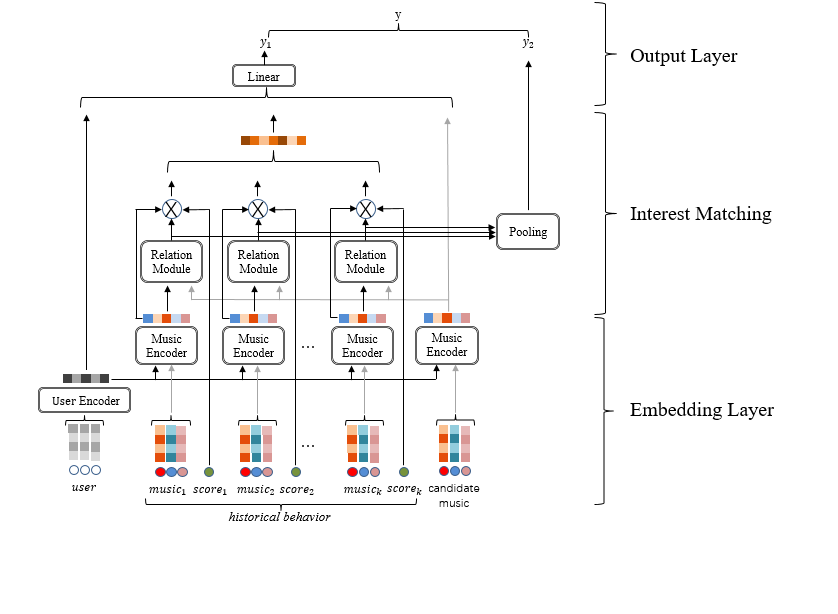
\includegraphics[width=15cm]  {MusicRecomSurvey/pics/model_final.PNG}}    
\caption{\label{4} 模型结构图}      
\end{figure}

详细的模型介绍将在之后的实验方案改进说明中给出。

\subsubsection{程序设计方案}
我们通过Python和PyTorch等开源库,搭建了我们的数据处理模块,以及神经网络结构。具体的设计思路在附录X中。
%\subsection{数据集处理}
\subsubsection{数据筛选}
经过对数据的初步查看,我们发现我们的数据集中虽然规模较大,但是其中的噪声比较大,所以我们对于数据集进行了一步初筛。首先,我们筛除了交互数据数量少于10的用户以及音乐。来保证训练集中的样本信息足够充分。同时我们简单筛除了一部分微信中微商的信息,这部分用户及其文本信息我们认为并不能表现出太大的价值。经过这样的一轮筛选,我们得到的数据集有181137个用户,38306首音乐,15258008项交互数据。我们的数据集和其他相关的数据集的比对如表2所示:

\begin{table}[htbp]
\centering
\caption{不同数据集的情况}
\begin{tabular}{|l|l|l|l|}
\hline

Dataset & Users & Items & Samples \\ \hline
Amazon(Electro) & 192,403 & 63,001 & 1,689,188 \\ \hline
MovieLens\cite{Harper:2015:MDH:2866565.2827872} & 138,493 & 27,278 & 20,000,263 \\ \hline
Ours & 181,137 & 38,306 & 15,258,088 \\ \hline

\end{tabular}
\end{table}

\subsubsection{音乐行为处理}
我们将分享和收藏的行为计10分;收听按照时长和总时长的比例积分,完整收听计为5分;摇一摇计为5分。综合计算上面的所有得分,对于高于6分的交互记为正例。

\subsubsection{特征选取}
经过一些测试,我们选定了如下的用户及音乐特征,这些特征信息均能在我们的数据集中得到:
\begin{itemize}
    \item 用户:性别、年龄、省份、文章阅读、朋友圈文本
    \item 音乐:歌手、流派、歌词、音频
\end{itemize}


\subsubsection{数据集构建}
接下来,我们要对数据集进行分类,划分出正负例,以及训练集和测试集。在上面的形式化描述中,我们将问题定义为一个二分类的问题,所以这里我们也采取二分类的方式进行选取。根据上面对于音乐行为的处理评分,我们将高于6分得分的音乐记为正例,这表明所有分享和点赞的音乐均为正例,完整收听并不会被记为正例,但是如果还有摇一摇等行为,则表明用户有一定的兴趣去主动查找对应的音乐,此时则被记为正例。

接下来需要选取负例。我们选择使用负采样的方法进行负例选取:随机在负例样本中选取和正例数量相同的负例,来保证样本分布尽量均衡。但是,什么样的样本算是负例,就是我们需要考虑的问题了。首先我们将低于6分的样本记为负例,在其中进行随机采样。但是经过一些实验和预训练,我们发现这样训练得到的模型的效果并不好。之后,我们经过讨论认为不能将分数小于6分的音乐视作负例。因为有评分的音乐表明用户和这个音乐有一定的交互行为,虽然没有表现出明显的兴趣,但是这种交互行为表现出了一个正向的倾向。所以我们认为将这部分设置为负例是不合适的。经过调整过后,我们将用户未进行评分的音乐作为负例集合,在其中进行随机采样。虽然这部分的音乐中可以看作是含有用户感兴趣的内容的,但是我们认为相比于这些感兴趣的内容,在这部分音乐中用户不感兴趣的内容数量是更多的。所以这样的采样有很大的概率采样得到的就是不喜欢的内容了。

完成正负例的判定和选取之后,我们歌曲按照4:1的方式对于训练集和测试集进行划分,保证测试音乐只在测试集中出现。此时在训练过程中就不会出现这些测试集的音乐,因此在测试时,这些音乐相当于全新的音乐,成功模拟了冷启动的情况。此时,有30645首歌曲在训练集中,7661首歌曲在测试集中。
%\subsection{Baseline}
为了比对不同算法模型和我们的模型之间的性能差异,我们选择了一些在推荐系统中用到的方法作为Baseline,在我们的数据集上进行了测试,具体的Baseline如下:
\begin{itemize}
    \item Neural Collaborative Filtering(NCF)\cite{he2017neural}:神经网络协同过滤。使用神经网络方法对传统的协同过滤算法进行扩展。
    \item DeepInterest Network(DIN)\cite{zhou2018deep}:从用户历史交互数据中抽取用户兴趣,实现物品与兴趣之间的匹配。
    \item DeepFM\cite{guo2017deepfm}:将因子分解机(Factorization Machine, FM)中的部分结构使用神经网络进行扩展。使用因子分解机获取低阶组合特征表示,神经网络获取高阶组合特征表示,综合使用这些特征信息进行推荐。
    \item xDeepFM\cite{lian2018xdeepfm}:DeepFM的改进版,将DeepFM中的因子分解机替代为Compressed Interaction Network(CIN),利用CIN获取高维特征组合
\end{itemize}
上面的若干模型是近些年来使用神经网络进构造推荐系统中较为经典的结构,但是为了使其能够正常处理冷启动的情况,我们在这些模型的基础上结合了DropoutNet\cite{volkovs2017dropoutnet}。DropoutNet是针对于冷启动问题提出的模型,该模型在输入时舍弃了latent factor的信息,来模拟冷启动的场景。与上面的若干模型结合,能够使其对于冷启动场景能够更好地适应。

为了评价不同的模型,我们选取了两个评价指标。首先是AUC,其中$rank_{i}$表示第$i$条样本得分的排序,$M$和$N$分别为正负样本的数量。
\begin{equation}
    AUC = \frac{\sum_{ins_i \in positive} rank_{ins_i} - \frac{M(M+1)}{2}}{M \times N}
\end{equation}

此外还有准确率指标Accuracy:
\begin{equation}
    Accu = \frac{\#\{CorrectSet\}}{\#\{TestSet\}}
\end{equation}
%\subsection{实验结果}
经过测试,我们在自己的数据集上对于不同的模型进行了测试得到的结果如下:
\begin{table}[htbp]
\centering
\caption{冷启动实验结果}
\begin{tabular}{|l|l|l|l|}
\hline

Methods & Accu & AUC \\ \hline
NCF &  0.5000 & 0.5092 \\ \hline
DropoutNet+DIN & 0.6206 & 0.6634 \\ \hline
DropoutNet+DeepFM & 0.5796 & 0.6999 \\ \hline
DropoutNet+xDeepFM & 0.6027 & 0.7112 \\ \hline
Ours & \textbf{0.6547} & \textbf{0.7249} \\ \hline

\end{tabular}
\end{table}

从上面的表格中,我们可以得到一些结论。首先,对于非基于内容的模型NCF,其是通过交互信息来对评价进行预测的,所以在面对音乐的冷启动场景时,并不存在这样的交互信息,所以无法正确进行工作,所以该模型在本数据集上的准确率是0.5000,相当于随机猜测。在这样的冷启动问题中,如何对于全新的音乐给出特征上的表示和描述就是关键的步骤了。从实验的结果中可以看出,我们基于用户信息的音乐特征表示是优于其他的方法的,从而在冷启动数据上的两个指标中均能取得更好的结果。

接下来,我们希望查看我们的模型在非冷启动场景下的表现。所以我们将模型在非冷启动的数据集上进行测试,得到如表4的结果:

\begin{table}[htbp]
\centering
\caption{非冷启动实验结果}
\begin{tabular}{|l|l|l|l|}
\hline

Methods & Accu & AUC \\ \hline
DIN & 0.9009 & 0.9630 \\ \hline
Ours & 0.9156 & 0.9689 \\ \hline

\end{tabular}
\end{table}

可见我们的模型在非冷启动的状况下也能取得优于其他模型的表现。

另外,我们还通过另外一组实验验证了我们的模型在面对Feature缺失情况下的表现。得到的结果如表5:
\begin{table}
\centering
\caption{Feature缺失实验结果}
\begin{tabular}{|l|l|l|l|}
\hline

Missing Feature & Accu & AUC \\ \hline
音乐风格 & 0.6504 & 0.7176 \\ \hline
音乐音频 & 0.5957 & 0.6313 \\ \hline
音乐歌手 & 0.6333 & 0.7012 \\ \hline
用户ID & 0.6541 & 0.7193 \\ \hline
用户年龄 & 0.6417 & 0.7160 \\ \hline
用户性别 & 0.6464 & 0.7214 \\ \hline
用户阅读文章类型 & 0.6519 & 0.7206 \\ \hline
用户朋友圈文本 & 0.6469 & 0.7146 \\ \hline
未缺失 & 0.6547 & 0.7249 \\ \hline

\end{tabular}
\end{table}

通过这样的实验结果,我们可以评价各个Feature对于我们模型的“敏感程度”。比如对于音乐来讲,音乐风格缺失时的结果发生的变化很小,因为大多数的音乐都是“Pop 流行”类别的,所以很难通过音乐风格体现音乐的特征。而音乐音频,音乐歌手两项音乐的Feature对于模型有一定的影响,音乐音频的影响更大,这表明用户相比于歌手,考虑的更多的还是歌曲听起来的感觉。对于用户来讲,用户ID对于模型基本没有影响,用户的年龄,性别,阅读文章类型,朋友圈文本等内容均有一定的影响,但是影响并不算太大。为了比较我们的模型对于这些特征缺失的稳定性,我们选取了另一个模型来进行确实特征的测试,得到的比对结果如表6:

\begin{table}
\centering
\caption{xDeepFM与我们模型的Feature缺失性能}
\begin{tabular}{|l|l|l|l|}
\hline

Missing Feature & xDeepFM & Ours \\ \hline
用户id & 0.7213 & 0.7193 \\ \hline
用户年龄 & 0.7008 & 0.716 \\ \hline
用户阅读文章类型 & 0.6928 & 0.7206 \\ \hline
用户性别 & 0.7157 & 0.7214 \\ \hline
音乐音频 & 0.5253 & 0.6313 \\ \hline
音乐风格 & 0.6982 & 0.7176 \\ \hline
音乐歌手 & 0.6699 & 0.7012 \\ \hline
不缺失 & 0.7213 & 0.7249 \\ \hline

\end{tabular}
\end{table}

可见在用户ID上,xDeepFM性能更好,但是这一特征对于模型并不是特别关键。而对于其它的特征,我们的模型在特征缺失时的性能能够比xDeepFM好很多。
%\subsection{实验总结与展望}
在本次的实验当中,我们对于数据集中的内容进行了一些处理。其中对于正负例的划分,我们卡了很久,实验的效果一直没有明显的提升,经过一番讨论我们才发现评分低不代表没兴趣而是代表兴趣不高的这样的一个假设,经过实验测试,我们发现实验的结果有了较为明显的好转。此外,我们的数据在初始时并没有进行归一化,所以模型一度不会收敛,之后对模型实现进行排查,解决了这样的问题。

在下一步的工作当中,我们希望能够通过跨数据集的实验,来验证我们的模型在不同的实验数据级下的表现,来确定我们的实验模型是否是较为完备的。同时,我们目前的实验结果更多地是面向于实验数据的,并没有对于实验案例进行具体的分析。所以我们希望能够在下一步的工作中对于典型案例进行选取,进行case study,来表现我们的实验结果是确实满足推荐要求的。
%\subsection{Case Study}
通过我们的模型,我们对于不同的歌手之间的相关关系进行了一定的调研,选出了每个歌手最相似的歌手,结果如下:

周杰伦:周杰伦, 张国荣, 赵雷, 任贤齐, 黑龙, 李克勤, 庄心妍, 望海高歌, 张碧晨, 风语

张国荣:张国荣, 周杰伦, 许嵩, 赵雷, 黑龙, 张碧晨, 李健, 凤凰传奇, 任贤齐, 庄心妍

许嵩:许嵩, 凤凰传奇, 张国荣, 张碧晨, 周杰伦, 黑龙, 李健, 赵雷, 任贤齐, 庄心妍

汪峰:汪峰, 郑秀文, 邓紫棋, 崔子格, 网络歌手, 卫兰, 张津涤, 门丽, 蔡健雅, 冷漠

邓紫棋:邓紫棋, 汪峰, 郑秀文, 卫兰, 崔子格, 网络歌手, 蔡健雅, 郑源, 张津涤, 门丽

五月天:五月天, 杨千嬅, 杨坤, 祁隆, 张玮伽, 张杰, 谭咏麟, 张宇, 秋裤大叔, 水木年华

杨坤:杨坤, 五月天, 周传雄, 水木年华, 张杰, 望海高歌, 汪苏泷, 谭咏麟, 杨千嬅, 李克勤

可见,对于歌手之间的相关关系,我们并不能找出特别明显的关联,但是仍然可以部分描述歌手与歌手之间的风格相似程度。比如许嵩和周杰伦的距离较近,而许嵩在早期以翻唱周杰伦起家,风格势必有一定的相似性。同时,汪峰和邓紫棋的曲风也有一定的相似性,杨坤和五月天的音乐风格也是相似的。这表明我们的模型能够从某种层面上对于歌手,歌曲特征进行抽象,但是这种抽象的可解释性较差,很难找到特别明显的特征信息。
\section{实验方案改进说明}
由于我们并不是先实现了另外的模型再在此基础上进行改进,而是直接对我们的模型进行设计和搭建的,所以在本部分的内容中,我们将对于我们的模型结构和设计思路进行详细的介绍。
\subsection{模型结构}
模型结构图如图9所示。
\begin{figure}[htb]        
\center{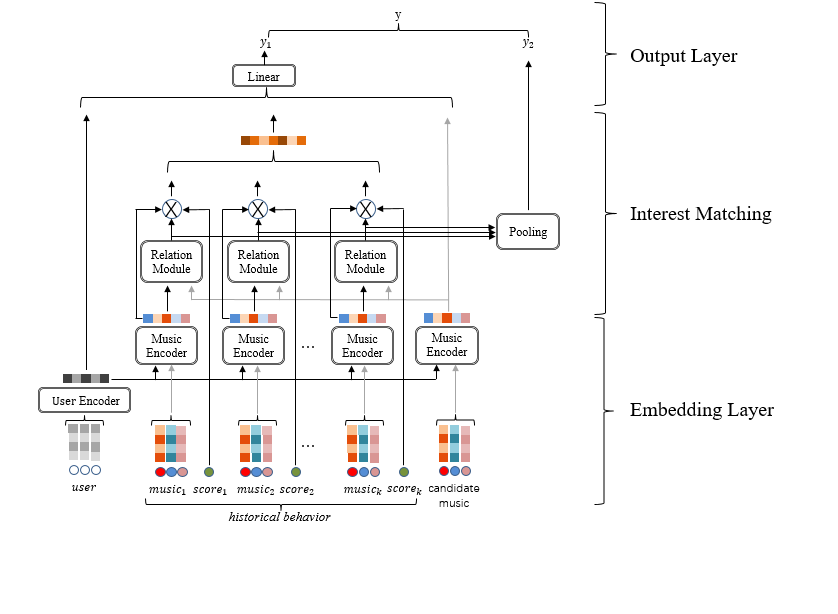
\includegraphics[width=15cm]  {MusicRecomSurvey/pics/model_final.PNG}}    
\caption{\label{4} 模型结构图}      
\end{figure}

\subsubsection{Embedding Layer}
根据我们的数据集,我们可以获得若干的特征,我们将特征先通过线性层或者Embeding层进行编码,得到一系列特征的向量表示。接下来就是根据这些向量,对于用户及音乐进行编码。下方的user表示目标用户的若干特征,用向量表示。将其作为输入,经过User Encoder,得到对于用户特征的编码向量。接下来,对于一些用户已经评分过的音乐,我们知道这些音乐的特征和评分,我们将特征和用户的特征向量结合在一起,分别输入到Music Encoder中进行编码,此时能够结合用户对于音乐的个性化信息,从而相同的音乐对于不同的用户来讲,经过Music Encoder得到的编码是不同的。对于待评价的音乐,我们只有他们的特征值,但是仍然可以像已知评价的音乐那样,通过Music Encoder,获得其特征向量。这部分就是音乐的编码层Embedding Layer。具体地,两种Encoder的结构如图10所示,可以见到Encoder的主要结构是Multi-Head Attention\cite{vaswani2017attention}模块,其结构如图11所示。

关于音乐选取的数量,我们也进行了一定的调整。我们在输入时需要有一系列已知评分的特征以及其最终的评分,但是一个人的历史记录会有很多条,并且数量各不相同,而我们的模型结构并不支持对于输入数量动态进行调整,所以我们选择使用采样的方法,每次训练时,从用户的历史音乐中选取5首历史评价过的歌曲进行输入,经过多轮训练后,基本能够将所有的评价歌曲均利用在训练当中。这种方法虽然对数据集的利用效率不高,但是能够较大地降低训练的时间成本和模型的复杂度,所以我们经过权衡,选择了随机选取5条数据的方法。

\begin{figure}[htbp]        
\center{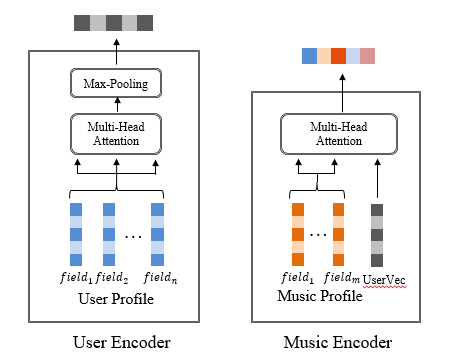
\includegraphics[width=10cm]  {MusicRecomSurvey/pics/model_encoder.PNG}}    
\caption{\label{4} Encoder结构}      
\end{figure}

\begin{figure}[htbp]        
\center{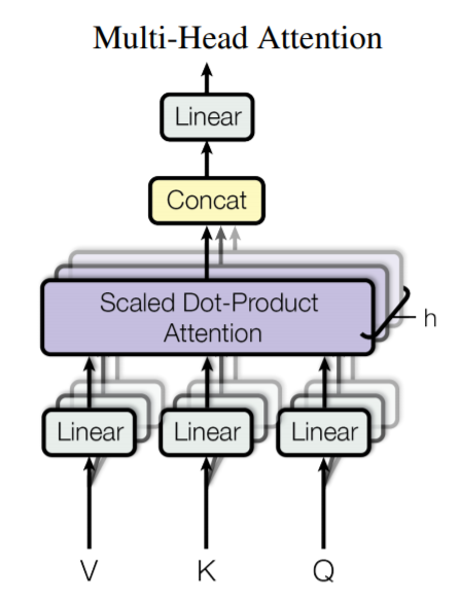
\includegraphics[width=7cm]  {MusicRecomSurvey/pics/Multihead.png}}    
\caption{\label{4} Multi-Head结构}      
\end{figure}


\subsubsection{Interest Matching}
\begin{figure}[htbp]        
\center{
\includegraphics[width=7cm]  {MusicRecomSurvey/pics/relation_module.png}}    
\caption{\label{4} Relation Module结构}      
\end{figure}

之后我们根据若干已评价的音乐和一个待评价音乐的特征向量,通过一个Relation Module,具体结构如图12所示。通过这样的结构,可以对于这些音乐之间的相似度进行预测,其得到的结果就是已知评分音乐和未知评分音乐之间的相似程度。事实上,我们的Relation Module并不算特别复杂,需要训练的参数只有一个矩阵$W$,事实上,我们也使用更加深层的结构替换本结构进行了测试,但是发现这样做不仅会增加训练时间和参数规模,并且得到的准确度也会下降一些,所以最终我们还是选择了将两向量关于$W$求内积之后再进行$sigmoid$得到0\~1之间的值作为相似程度。

根据相似度,我们将根据已知评分音乐的相关特征,构造处待预测音乐的特征。方法就是加权平均,每一项的权值是得分乘上相似度,从而,越相似的音乐,以及得分越高的音乐,对于预测结果的影响就越明显。最后得到特征向量的一个估计值。

\subsubsection{Output Layer}
最后就是一个Output Layer输出层,综合之前给出的两项评分结果,给出最后的结论。第一部分的结论$y_1$有由之前的用户编码,待预测音乐估计特征,待预测音乐编码等内容过一个线性层,得到的结果,这部分体现处了协同过滤思想中根据相似度和评分得到目标评分的思想。另一部分结论$y_2$得到的方法是通过一个Max Pooling层,选取出相关性最大的值。这部分体现出的策略是当待预测歌曲和之前的历史歌曲有很高的相似性时,我们认为用户很有可能对于待评价歌曲有一定的兴趣,所以此时该结果是一个较大的相似度的值。最后,我们将两个评分制取平均,得到最终的输出。这是一个0\~1之间的值表示用户可能感兴趣的程度。

\subsection{模型创新点}
我们的模型对于这些问题进行了一定的讨论和修正。

首先,我们引入了Self Attention机制和Multi-head Attention机制\cite{vaswani2017attention},在编码层实现了用户个性化的音乐编码,即将用户的特征编码用于音乐的编码过程,这就保证了对于不同的用户,就算是相同的歌曲,其编码也是不同的。这就保证了推荐过程更加富有个性化。

此外,我们考虑了不同交互行为对于提取用户兴趣的不同贡献,给出了一套用户兴趣的评分系统,并在利用历史交互信息捕捉用户兴趣时,实现了对于特征的降噪处理。

同时,我们引入了比较学习的思路,基于比较用户以往喜欢的物品以及待判断物品的思路,挖掘深层次的特征,从而能够更好地捕捉用户兴趣。并最终取得了较好的实验结果,具体的结果比较将在后面的部分给出。
%\section{总结与展望}
%\subsection{肖朝军}
小组分工:模型架构搭建;新模型设计,实现与测试;DIN模型的复现与测试。

本次小学期我们小组选择了“社交媒体中的音乐推荐”一题。该项目主要涉及从人们社交媒体中的交互信息中获取相应的用户画像,提取用户兴趣,并为用户推荐相应的音乐。

由于具备神经网络相关的模型设计的经验,在本次项目中我主要负责了数据处理、baseline构建、自主模型设计等工作。为了保证项目选题可以得到圆满的完成,在整个小学期中,我对该项目投入了较大的时间。在前期阅读了大量的推荐系统相关论文之后,我们最终聚焦在推荐系统的冷启动问题上。

在进行文献调研工作时,我发现推荐系统作为目前应用及其广泛的系统,近几年来已经有非常非常多的学者关注到这样一个问题上,近几年光是运用神经网络方法来解决推荐系统问题的文章更是多达几百篇。这也就导致了在短时间内,我们无法对推荐系统的发展现状有一个全面的认识。因此在阅读了助教推荐的几篇文章并和助教沟通后,我们决定着重调研推荐系统冷启动这样一个方向。经过调研,发现研究冷启动问题的论文相对较少,我们也因此决定研究这样一个问题。

在着手实现相关模型时,由于对该领域不够熟悉,我们浪费了很多时间在数据处理上,在负例选取、数据归一化上耽误了很长一段时间,一度觉得自己要做不出来了。后来在助教的帮助下,在中期答辩前,顺利跑完了相关的实验,并验证了我们设计的模型的效果。

在设计模型时,我们主要将自然语言处理领域非常常用的self-attention机制与multihead-attention机制应用到推荐系统中,取得了一个非常不错的效果。因此,这也说明了在进行相关学术研究时,我们不应该局限在某一个狭小的领域,多阅读不同领域的文章可以很好地帮助我们开展相关的工作,并提供灵感。

总而言之,这次小学期项目设计中,遇到了很多的困难,也迸发了很多灵感。我认识到了我许多的不足,在未来的学习过程中,我将注重培养个人的发现问题能力、实验方案设计的能力,努力做出有影响力有意义的学术工作。
感谢助教和老师在本次项目完成中,给我们小组提供的帮助!

\subsection{曹晨阳}
小组分工:Demo架构与经典方法的设计与实现;CML模型的复现;报告撰写。

经过几周的探索和实践,我们最终还是完成了这样一个音乐推荐系统,并取得了不错的成果。

在经过第一周的文献综述后,我们对于数据有一些初步的处理和认识,此时我们对于如何使用这些数据,如何构建我们的模型都充满了疑惑。在第二周,我们决定先从冷启动出发,探究是否有一些解决冷启动问题的思路。我们先后看了一些其他领域中关于冷启动的文章,像是关于Meta-Learning,Metric-Learning等领域,我们发现有些被用于其他领域如CV中的技术可能可以帮助到我们,所以我们逐步参考其他的模型,建立了我们基于Relation-Network的模型。之后就是实验设计等方面的内容了,其中的难点在之前的报告中已经进行了叙述。最后我们的模型在自己的数据集上比现有其他模型取得了更好的效果,说明我们的设计还是有一定的道理的。

之后是一些反思和展望。在快要结题的时候,我们小组的肖朝军同学发现了一篇文章,说当前推荐系统中广泛使用的神经网络方法其实是不必要,甚至有些方法是难以复现的,使用传统的方法也能达到相似的准确度。这也引发了我们小组的思考,我们开始更加注重对于其他baseline模型的复现,以及一些模型设计上的问题。最后的Case Study我们进行了一些工作,但是并不充分,有些可视化也没来的及做,还是有一些遗憾的。在答辩过程中,老师给我们组的意见是更加充分使用当前的数据集,我们认为还是有一些道理的。在最开始的调研当中,我们认为情绪确实能够影响到音乐的选择,但是朋友圈文本量大,图片获取也比较复杂,同时夹杂很多没有意义的文本,所以我们对于这部分的信息利用并不是特别充分,如果我们能够对于有效的朋友圈的情感信息进行分析,相信能够对我们的模型有更大的提升。

最后感谢贾老师和沈导在这几周内的悉心指导。

\subsection{张泽阳}
小组分工:NCF、DeepFM、xDeepFM模型的复现与测试。

在为期五周的小学期中,我们进行了文献综述、切入点探究、模型设计、baseline实现、case study等一系列工作。由于时间紧迫,无法更全面和深入地了解音乐推荐系统,我们选择了“音乐推荐系统中的冷启动问题”作为主要命题。一整套流程下来,对于科研方法有了一定的了解。

在本次项目中,遇到了很多的困难,同时这也伴随着很大的收获:
前两周文献综述的时候,看了大量文章,但始终类似于一个BFS的过程,看在眼里,觉得挺有道理,但是由于之前没有接触过这个领域和模型实现,也难以断定其优点与可改进之处。总觉得一个模型是理论上要体现出优越性,才能对实验有所期待,但实际上这会导致进度遥遥无期。快开题的时候,还是朝军同学敏锐地发现了Relation network 在本命题上的可改进性,一针见血地提出了其关于冷启动问题对症下药的优越性,让我们如期开题。

在实现NCF的过程中,一开始诧异于输入的数据只有id或者交互矩阵的行列,最后和同学交流才发现其本质上还是CF方法,只不过神经网络不同于传统方法如MF、FM等,能学到更高阶的关系。看NCF论文的时候,看到过他们采用了负采样的方法,没多在意。后来和助教沟通才发现,我们的模型AUC很低,是由于我们对于数据本身的理解出现了偏差,在采用负采样之后,终于在报告前回归正常水平。当AUC比较低的时候,本能地想是不是参数不太对,浪费了许多时间在调参上,而实际上数据利用、模型的训练技巧上更值得考究。我感到,模型实现和积极交流能使得研究者对于论文思想的理解更加深刻。

在几次报告中,老师和助教给我们提出了一些建议。我感到,模型具体的参数、指标可能并不是特别重要,而重要的是模型背后的故事——要改进什么?怎么改进的?为什么改进了?我想,这也分别是文献综述、模型设计、case study所要面临的问题。通过团队的合作努力,以及老师助教们的帮助与建议,我觉得我们在这些方面都做了很多,也学到了很多。

总而言之,本次小学期使我受益匪浅,同时也让我意识到之前自身研读论文不深不广、模型实现和方案设计都经验不足、发现问题的能力也有所欠缺。希望以后能在自己追逐的方向上做得更好。
十分感谢一起合作的队友、辛勤付出的老师和助教们!

\bibliographystyle{ieeetr}
\bibliography{ref}

%\section*{附录}
%\subsection*{附录1:程序设计报告}
%\subsection*{附录2:Demo设计报告}
%\subsection*{附录3:程序代码}
%全部的代码均在Github:https://github.com/Caochy/MusicRecom

%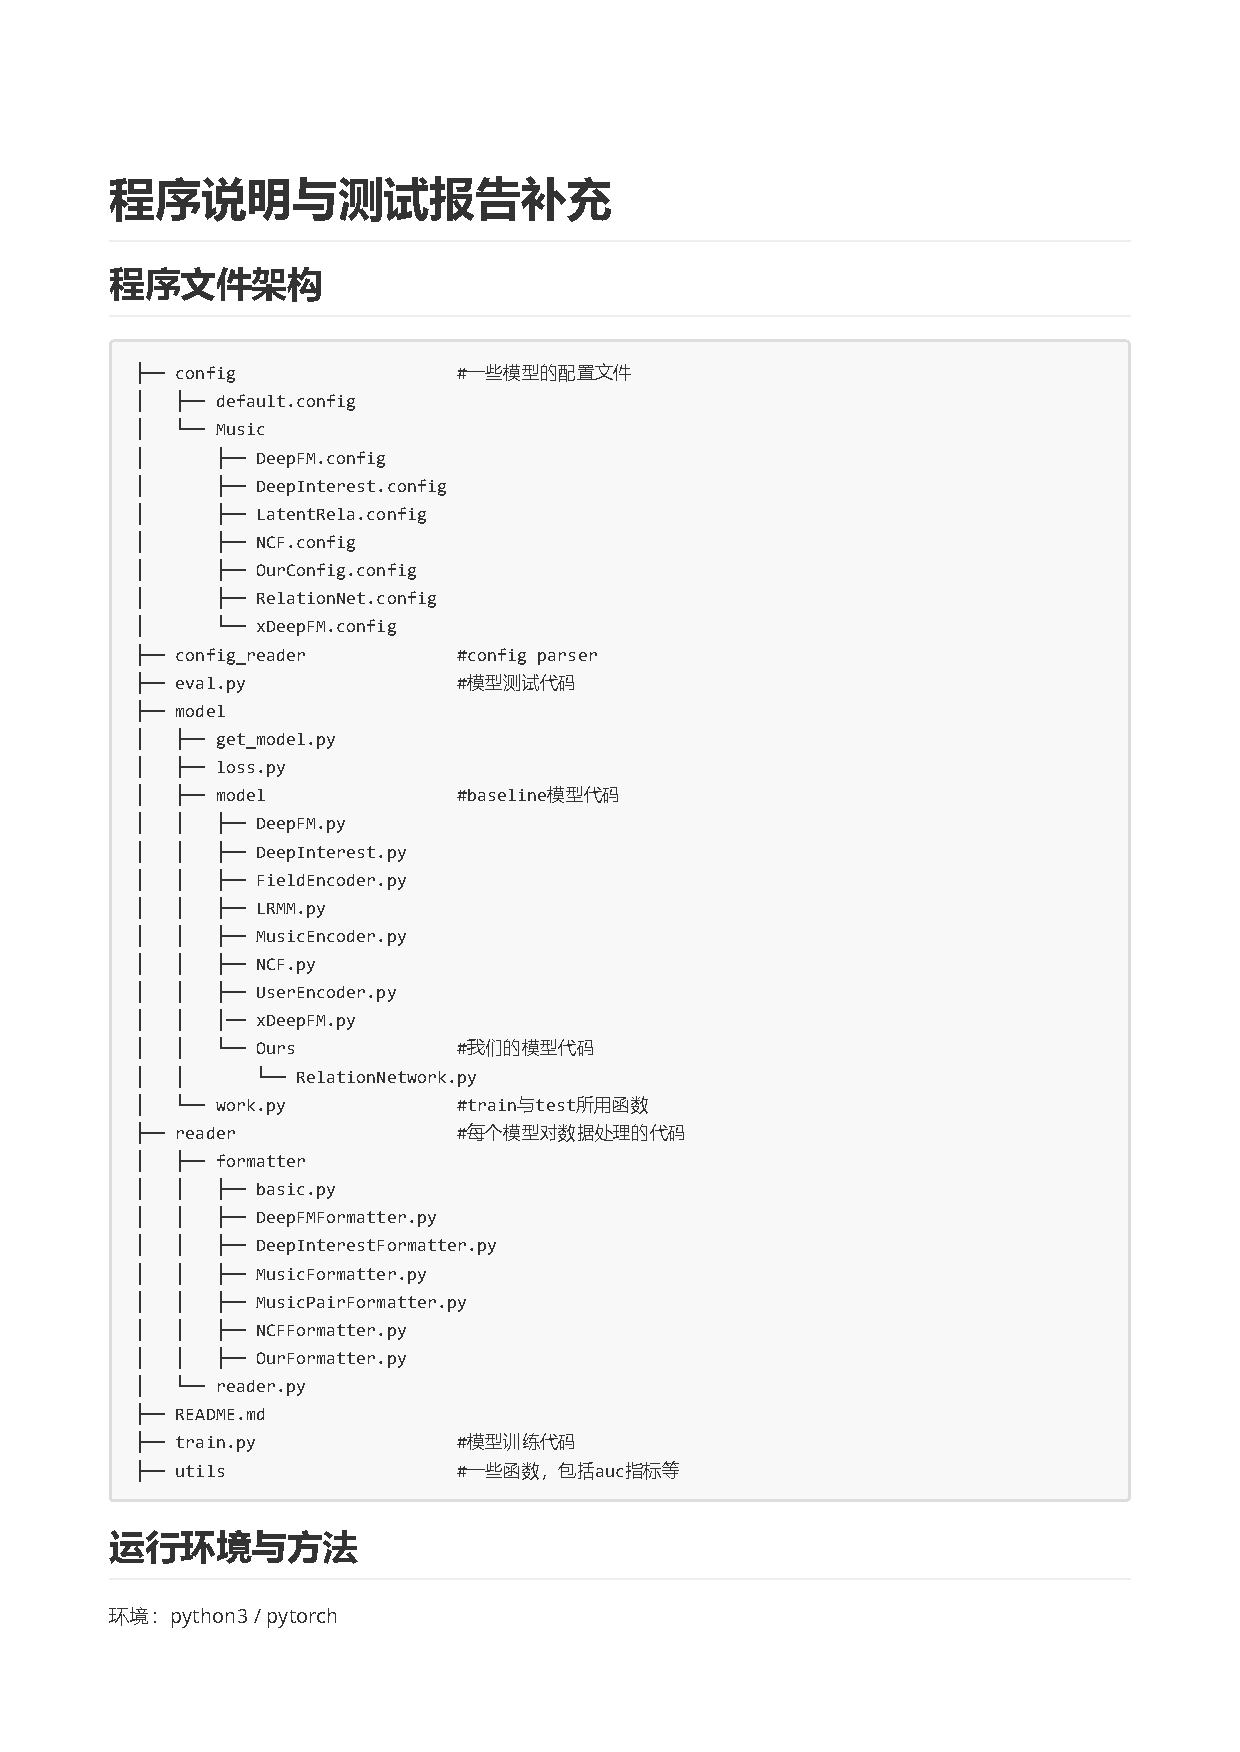
\includepdf[pages={1,2,3}]{data/readme.pdf}
%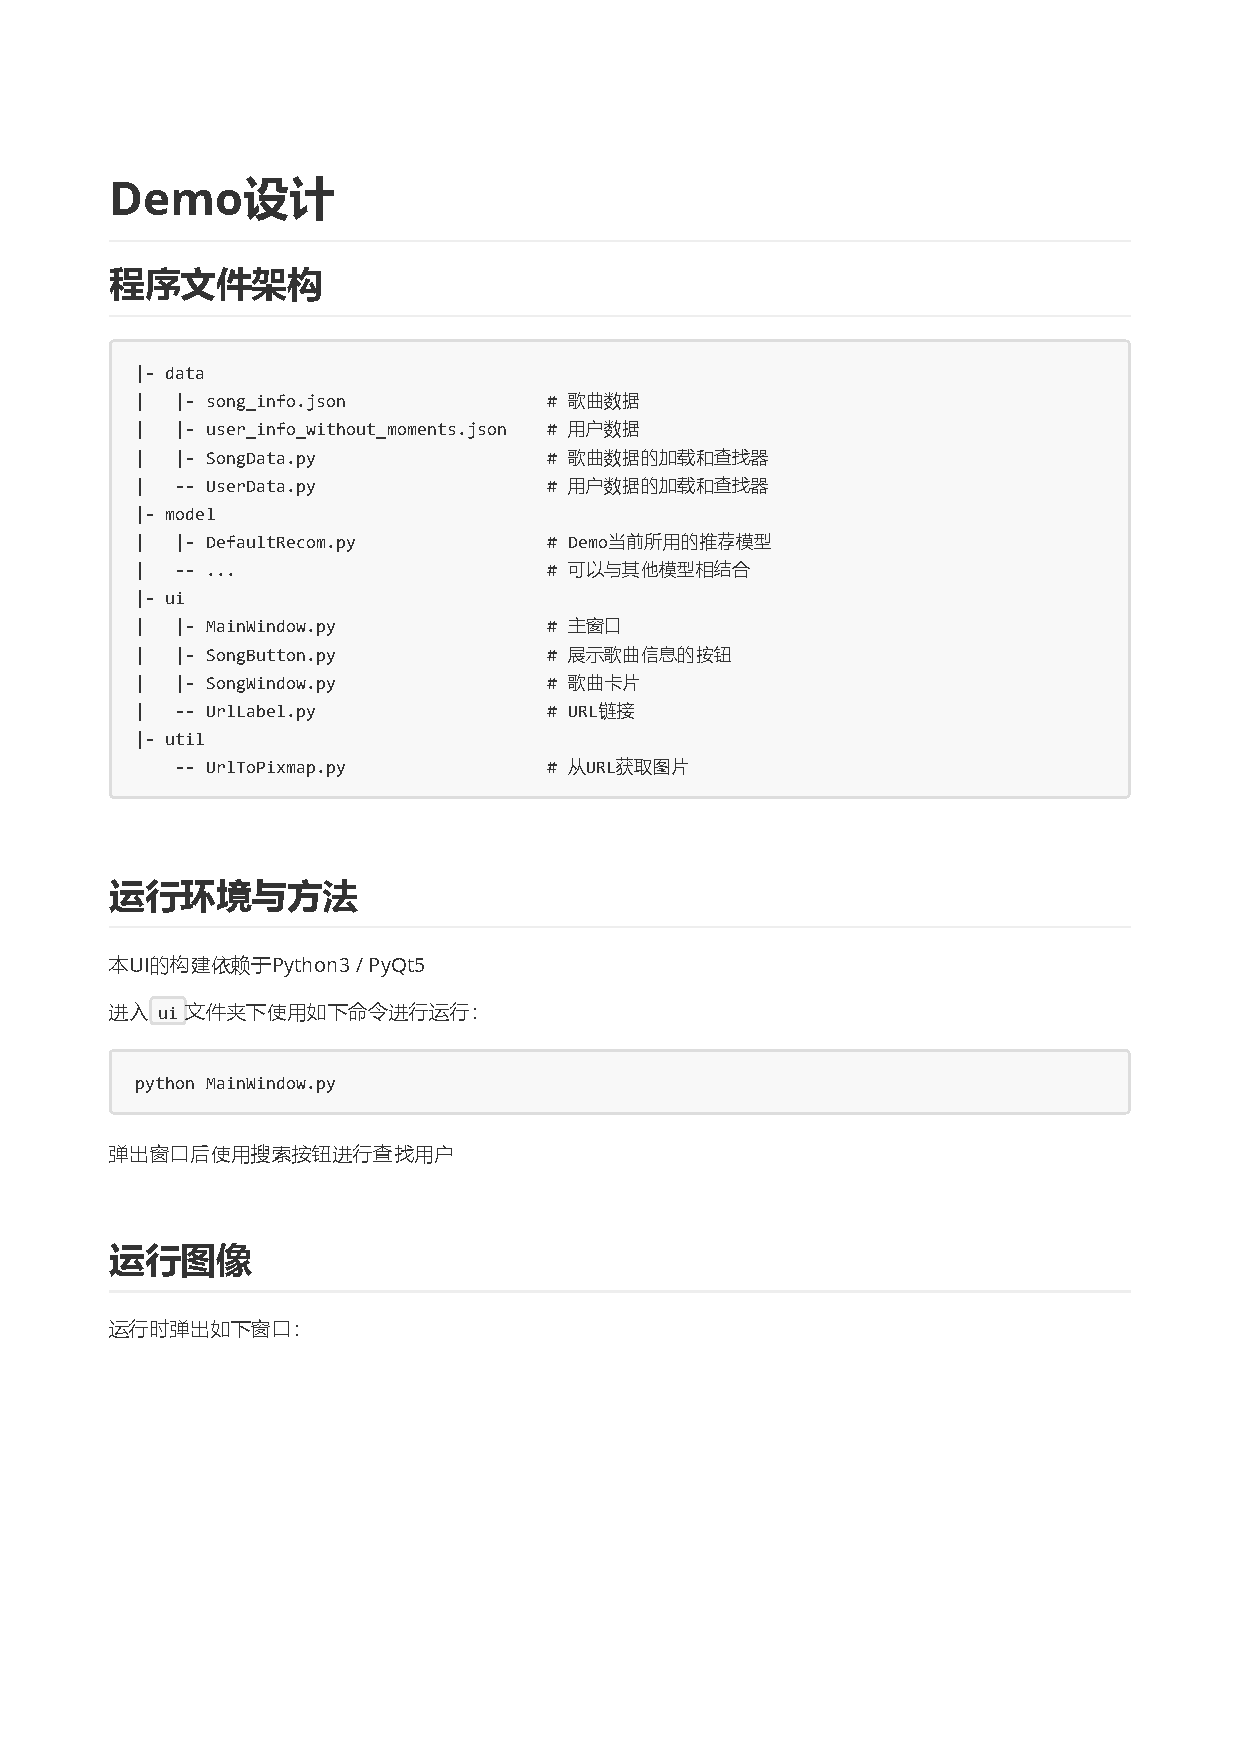
\includepdf[pages={1,2,3,4}]{data/demo_readme.pdf}
\end{document}
%结束
